\documentclass[	a4paper,
			11pt,
			oneside,
			parskip]{scrartcl}
\usepackage{package/ownstil}
\usepackage{package/owncmd}

\begin{document}
	
\setlength{\parindent}{0pt} 
\onehalfspacing

%--------------------------------------------
% Inhaltsverzeichnis
\tableofcontents 
\newpage
%--------------------------------------------

\section{Rahmenbedingungen und Zielstellung}

In diesem Projekt geht um die Realisierung eines Smartcard-basierten Ticketsystems für öffentliche Verkehrsmittel. Am Beispiel der U-Bahn soll es möglich sein Tickets nicht nur auf der Karte zu speichern, sondern auch die Bezahlung vorzunehmen. Hierzu kann der Fahrgast über die integrierte Geldkarte bezahlen oder mittels gesammelter Bonuspunkte für Vielfahrer. Des Weiteren soll es möglich sein den Fahrgast auf seiner Fahrt zu kontrollieren. Wurde das Ticket bereits beim Einlass kontrolliert und bestätigt, bleibt das Risiko das die Karte entwendet wurde. Ein Kontrolleur kann so während der Fahrt die Person anhand ihrer hinterlegten Daten und einem Bild, welches aus Platzgründen als Binärbild gespeichert wird, identifizieren. Aus Sicherheitsgründen wird die Übertragung verschlüsselt, somit ist es nicht möglich durch einwirken Dritter das Verhalten der Karte zu verändern.

\section{Entwicklungsumgebung}

Nachfolgend werden alle eingesetzten Hilfsmittel zur Erstellung der On- und OffCard Anwendungen aufgeführt und erklärt. Hauptrolle spielen hierbei JCIDE für die Entwicklung der OnCard Applets und Eclipse zur Erstellung der OffCard Anwendung auf Basis von JavaFX.

\subsection{E(fx)lipse}

Um die OffCard Anwendung mit JavaFx entwickeln zu können wurde von uns Eclipse verwendet. Da in der aktuellen Version noch keine Integration von JavaFX durchgeführt wurde, kann es mit Hilfe des Plugins e(fx)lipse um die nötige Funktionalität erweitert werden. \medskip

Die Vorzüge von JavaFX liegen unter anderem im neuartigen Aufbau der Benutzeroberfläche. Diese wird als FXML-Datei aufgebaut und ist somit isoliert vom restlichen Programmcode. Zusätzlich können die UI-Elemente über CSS-Datei optisch verändern werden. Auch hier bietet e(fx)clipse eine sehr attraktiven FXML und CSS-Editor, welcher Vorschläge gibt welche Attribute angewendet werden können, um ein Element zu definieren. 

\subsection{Package SmartcardIO}

Das Package SmartcardIO definiert eine Java-API für die Kommunikation mit SmartCards. Es ermöglicht den Java-Anwendungen mit Applets der SmartCards zu interagieren, um so Daten auf der Karte zu speichern und abzurufen. Eine \textit{TerminalFactory} erkennt alle angeschlossen Terminals und stellt eine Verbindung zur Karte her. \medskip

Über den Klasse \textit{CommandAPDU} lässen sich dann die zu übermittelnden Daten festlegen, inklusiver aller erforderlichen Parameter (CLA, INS, ...). Das sSenden des Befehls geschieht über die verbundene Karte und der Funktion \textit{getBasicChannel().transmit()}. \medskip

War das Senden erfolgreich, erhält man die \textit{ResponseAPDU} und kann diese über \textit{getData()} auswerten.

\subsection{JCIDE}

JCIDE ist eine Entwicklungsumgebung, die speziell für die Javacard-Programmiersprache entwickelt wurde. Das Entwicklungskit erlaubt es schnell und einfach JavaCard Applets mit den integrierten Tools zu erstellen. Der Grund für die Verwendung der IDE liegt in der Bereitstellung eines virtuellen Kartenlesegerätes. Nach dem Übersetzten des Applets erlaubt es die Anwendung die resultierende CAP-Datei automatisch mit dem Simulator zu verknüpfen. Das verhalten ist gleich einer echten JavaCard. Über das virtuellen Kartenlesegerät, können alle PC/SC kompatiblen Anwendungen mit dem Smartcard-Simulator kommunizieren. \medskip

\begin{figure}[H]
	\centering
  	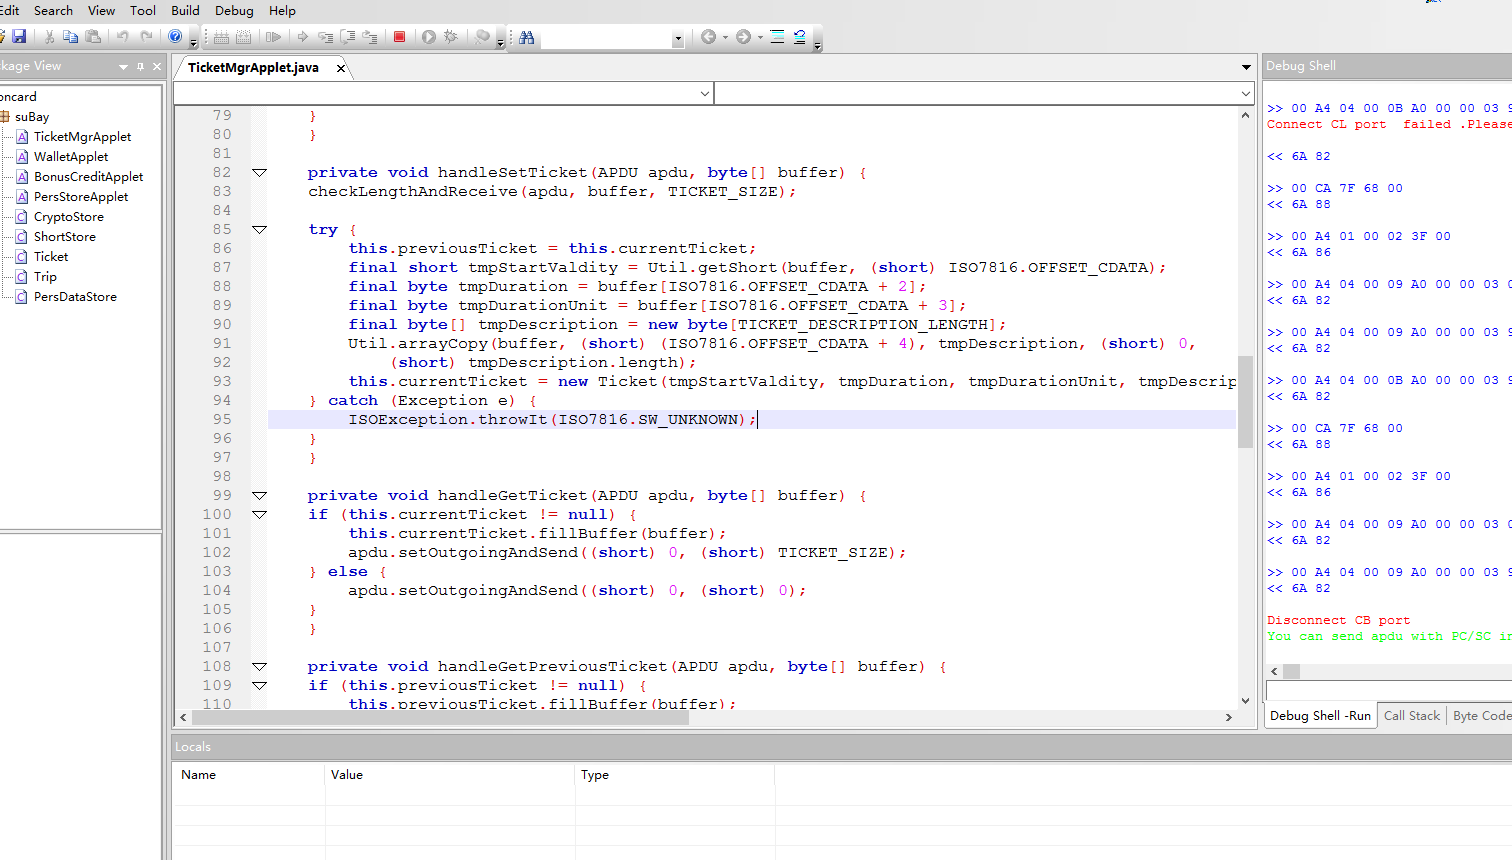
\includegraphics[width=0.9\textwidth]{img/jcide}
	\caption{JCIDE mit geöffneter Shell}
	\label{jcide}
\end{figure}

JCIDE wird von JAVACOS Technologies\footnote{http://www.javacos.com/developmentkit.php} entwickelt und auf einen aktuellen Stand gehalten. Allerdings ist die Installation nur  Windows-Systemen vorbehalten. \medskip

Weitere Vorteile bietet der integrierte Debugger, mit dem es möglich ist an jeder beliebigen Stelle Breakpoints zu setzen und somit schrittweise die Belegung aller Variablen zu zeigen.
Das Ausführen von Befehlen über die Debug-Shell ist ebenfalls möglich und ähnelt der Ausführung in Eclipse mit JCOP-Plugin. \medskip

Ein zusätzliches Tool (ebenfalls im Paket enthalten) ermöglicht die vereinfachte Kommunikation mit der Karte. Das als \glqq PyApduTool\grqq\/ bezeichnete Programm lädt die CAP-Datei aus dem Projektorder und zeigt alle gefundenen AID's auf. Somit entfällt die Eingabe des select-Befehls. Weiterhin existiert eine Ansicht, welche den send-Befehl übersichtlich aufteilt. Für jedes Byte existiert ein eigenes Eingabefeld. Diese Hilfe beugt Fehleingaben vor und speichert zusätzlich alle getätigten Operationen.

\subsection{SceneBuilder}

Der SceneBuilder unterstützt das Erstellen der FXML-Dateien zum Aufbau der Benutzeroberfläche. Alle unterstützen JavaFX UI-Elemente sind integriert und lassen sich per \glqq Drag and Drop\grqq\/ zur Bearbeitung in die eigene GUI einfügen. Die Darstellung wird permanent aktualisiert, somit ist jederzeit die konkrete Benutzeroberfläche ersichtlich. Ferner lassen sich alle Attribute zum ausrichten und beeinflussen der einzelnen Elemente direkt im Editor bearbeiten. Das Hinzufügen von IDs erleichtert zusätzlich den späteren Zugriff im Programmcode. Durch Annotations (@FXML) über den jeweiligen Variablen schafft die benötigte Verbindung.

\begin{figure}[H]
	\centering
  	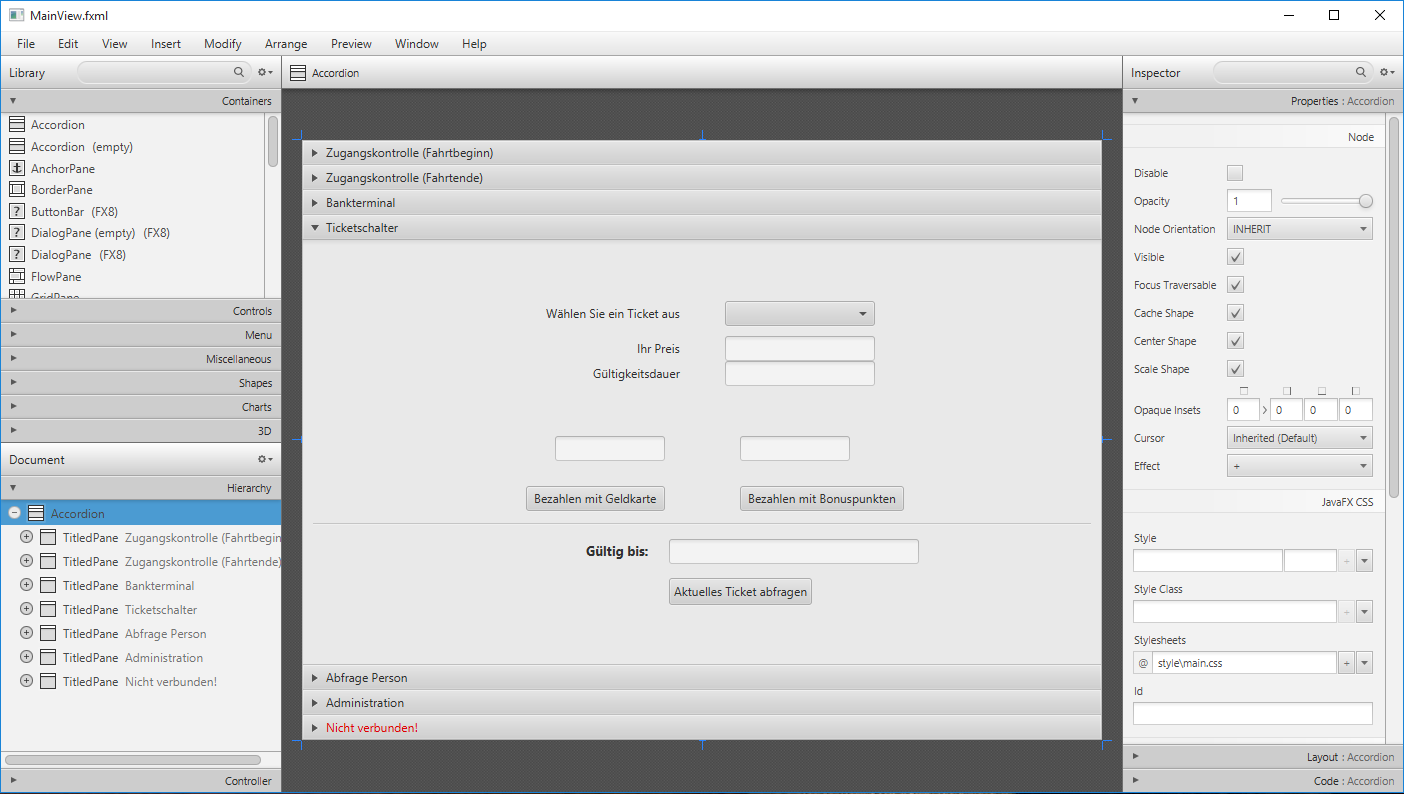
\includegraphics[width=0.9\textwidth]{img/scenebuilder}
	\caption{SceneBuilder}
	\label{scene}
\end{figure}

\subsection{GitHub}

Alle Programmteile sind öffentlich auf GitHub\footnote{https://github.com/philippsied/smartcard-course} zu finden. Neben den On- und OffCard Anwendungen ist auch diese Dokumentation  zu finden. Somit ist das Projekt für jeden zugänglich und verständlich.

\section{Programmcode}

In diesem Punkt geht es um die Erklärung der einzelnen Bestandteile des Projektes. Unterteilt in einen OnCard und einen OffCard Bereich werden die nötigen Schnittstellen erläutert, sowie die Funktionsweise der Programme erklärt. 

\subsubsection{Geldkarte}

Die Geldkarte dient dem Bezahlen der Tickets und musste somit vor dem Ticketsystem realisiert werden. In der ersten Phase genügte es die grundlegenden Funktionen zu implementieren, hierzu gehört das Aufladen, Abbuchen sowie das Abfragen des Kontostandes. Im späteren Verlauf gehört die Integration einer Verschlüsselungsmethode, um die Aufladung durch Unbefugte zu vermeiden.

\paragraph{OnCard} Zum Speichern des Geldbetrages wurde ein short-Wert definiert. Somit ist es möglich maximal 65536 Cent zu speichern. Dieser Betrag reich für die Geldkarte vollkommen aus, da ein Verlust der Karte, auch den Verlust des Geldbetrages bedeuten würde.

\begin{table}[H]
  \centering
  \caption{Klassenbyte und AID}
    \begin{tabular}{rr}
    \toprule
    \textbf{CLA} & \multicolumn{1}{l}{E0} \\
    \midrule
    \textbf{AID} & FD 75 42 61 79 57 61 6C 6C 65 74 \\
    \bottomrule
    \end{tabular}%
  \label{tab:walletaid}%
\end{table}%

\begin{table}[H]
  \centering
  \caption{Funktionsübersicht}
    \begin{tabular}{crcc}
    \toprule
    \textbf{Daten} & \multicolumn{1}{c}{\textbf{Größe}} & \textbf{Funktion} & \textbf{INS} \\
    \midrule
    Geldbetrag & \multicolumn{1}{c}{short} & aufladen & 0x10 \\
          & \multicolumn{1}{c}{} & abbuchen & 0x20 \\
          & \multicolumn{1}{c}{} & prüfen & 0x30 \\
    \bottomrule
    \end{tabular}%
  \label{tab:walletdata}%
\end{table}%

Bei dem Abbuchen eines Geldbetrages wird geprüft, ob der angeforderte Betrag mindestens dem aufgeladenen Guthabens entspricht. Bei einen zu hohen Geldbetrag wird die Aktion mit einer Exception (0x6A83) beendet. Auch das Überschreiten des maximalen Guthabens wird durch eine Exception (0x6A84) abgefangen.

\paragraph{OffCard} Die OffCard-Anwendung zum aufladen der Geldkarte fällt entsprechend der wenigen Funktionen des Applets sehr klein aus. Über eine ComboBox lässt sich ein entsprechender Betrag zum aufladen schnell auswählen und über die Schaltfläche \textit{Aufladen} zur Karte übertragen. 

\begin{figure}[H]
	\centering
  	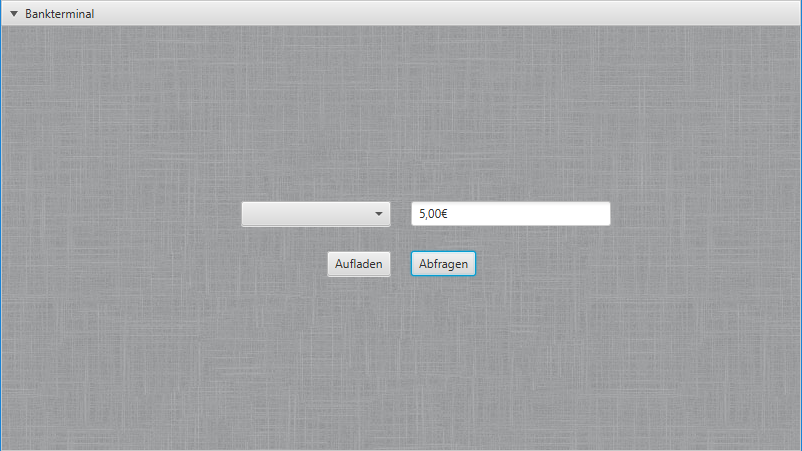
\includegraphics[width=0.9\textwidth]{img/wallet}
	\caption{Administration der Personendaten}
	\label{walletoff}
\end{figure}

Um den short-Wert in eine Byte-Folge zu konvertieren wurde mit der Klasse \textit{ByteBuffer} gearbeitet. Sie bietet die Möglichkeit beliebige Datentypen in eine Art Stapelspeicher abzulegen und als eine Byte-Folge bereitzustellen. Gleiches gilt für das entgegennehmen der Daten von der Karte. Die gelesenen Byte werden in den \textit{ByteBuffer} abgelegt und entsprechend der Datentypen herausgenommen. Zu achten ist auf die korrekte Reihenfolge der Informationen.

\subsubsection{Ticketsystem}

Das Ticketsystem ist fundamentale Grundlage für dieses Projekt. Nach der Implementierung der Geldkarte stehen der Entwicklung des Systems keine Hürden mehr im Wege. Des Weiteren soll durch die spätere Integration eines Bonussystems ein zweiter Zahlungsweg genutzt werden können. 

\paragraph{OnCard} Auf der Karte wird hierzu eine Beschreibung des Tickets, sowie die nötigen Zeiten für den Gültigkeitszeitraum des Tickets gespeichert.

\begin{table}[htbp]
  \centering
  \caption{Klassenbyte und AID}
    \begin{tabular}{rr}
    \toprule
    \textbf{CLA} & \multicolumn{1}{l}{E0} \\
    \midrule
    \textbf{AID} & FD 75 42 61 79 54 69 63 6B 65 74 4D 67 72 \\
    \bottomrule
    \end{tabular}%
  \label{tab:ticketaid}%
\end{table}%

Zum speichern einer Fahrt wird eine weitere Struktur benötigt. Diese hält alle Daten zum Antritt der Fahrt, wie den Zeitpunkt und den Namen der Station. Alle gespeicherten Zeiten werden bedingt durch ihre Größe (Unix-Zeitstempel) in zwei short-Variablen gespeichert. Die Aufteilung der int-Variabel findet allerdings in der OffCard-Anwendung statt.

% Table generated by Excel2LaTeX from sheet 'Tabelle1'
\begin{table}[htbp]
  \centering
  \caption{Add caption}
    \begin{tabular}{cc|rr}
    \toprule
    \textbf{Daten} & \textbf{Größe} & \multicolumn{1}{c}{\textbf{Funktion}} & \multicolumn{1}{c}{\textbf{INS}} \\
    \hline
    \textbf{Ticket} &       & \multicolumn{1}{c}{Aktuelles Ticket setzen} & \multicolumn{1}{c}{0x10} \\
    Beginn\_h & short & \multicolumn{1}{c}{Aktuelles Ticket abfragen} & \multicolumn{1}{c}{0x20} \\
    Beginn\_l & short & \multicolumn{1}{c}{Vorheriges Ticket abfragen} & \multicolumn{1}{c}{0x40} \\
    Ende\_h & short &       &  \\
    Ende\_l & short  &       &  \\
    Beschreibung & 30 Byte  &       &  \\
    \hline
    \textbf{Fahrt} &   & \multicolumn{1}{c}{Fahr - Startzeit setzen} & \multicolumn{1}{c}{0xA0} \\
    Beginn\_h & short & \multicolumn{1}{c}{Fahrt - Endzeit setzen} & \multicolumn{1}{c}{0xB0} \\
    Beginn\_l & short & \multicolumn{1}{c}{Aktuelle Fahrt anzeigen} & \multicolumn{1}{c}{0xC0} \\
    Station & 30 Byte &       &  \\
    \bottomrule
    \end{tabular}%
  \label{tab:ticketfunc}%
\end{table}%


\paragraph{OffCard} Die OffCard-Anwendung fällt bei diesem System größer aus. Wie in Abbildung \ref{ticketoff} zu sehen, wird anhand einer \textit{ComboBox} das gewünschte Ticket ausgewählt. Die restlichen Felder geben zahlreiche Informationen zum Ticket selbst, bzw. die Zahlungsmöglichkeiten mit dem jeweiligen vorhandenen Guthabens. Ist genügend Guthaben auf der Geldkarte vorhanden, so wird dem Fahrgast zugleich das neue Guthaben (nach dem Kauf) angezeigt. Gleiches gilt für die Bezahlung mit Punkten. \medskip

Bei Auswahl der Schaltfläche \textit{Bezahlen mit Geldkarte} wird zunächst auf das Applet der Geldkarte zugegriffen und der Kontostand kontrolliert. Reicht dieser aus, wird der entsprechende Geldbetrag abgehoben. War der Vorgang erfolgreich und die ResponseAPDU signalisiert dies, wird das Ticket generiert. Der Gültigkeitszeitraum und die Beschreibung des Tickets (Kurzstrecke, etc.) wird dann zur Karte als eine Einheit gesendet. Jederzeit kann der Fahrgast über die Schaltfläche \textit{Aktuelles Ticket abfragen} den Gültigkeitszeitraum der gekauften Fahrkarte abfragen.

\begin{figure}[H]
	\centering
  	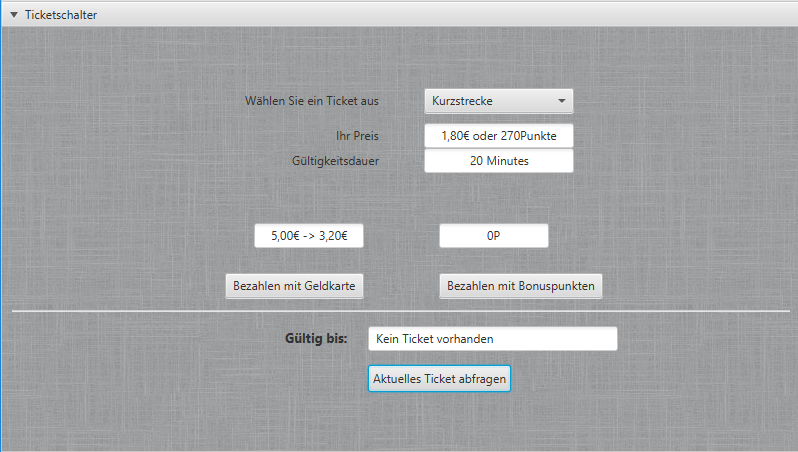
\includegraphics[width=0.9\textwidth]{img/ticket}
	\caption{Ticketschalter}
	\label{ticketoff}
\end{figure}

Zwei weitere OffCard-Anwendungen simulieren die Zugangskontrolle. Bei Fahrtantritt wird geprüft ob ein gültiges Ticket vorhanden ist. Ist dies der Fall, so \glqq öffnet\grqq sich die Zugangskontrolle und der Fahrtbeginn, sowie der Name der Station wird auf der Karte hinterlegt. Bei dem Beenden der Fahrt wird am Ausgangskontrolle die Fahrtzeit geprüft und mit der Gültigkeitsdauer des Tickets verglichen.

\begin{figure}[H]
	\centering
  	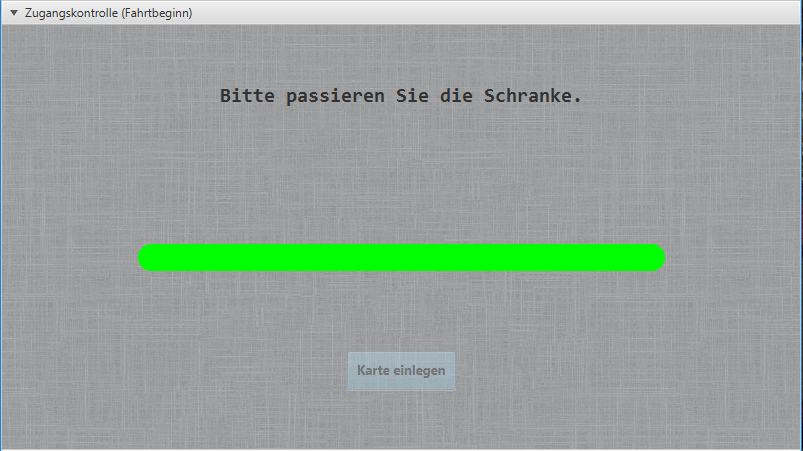
\includegraphics[width=0.9\textwidth]{img/gate}
	\caption{Zugangskontrolle}
	\label{gateoff}
\end{figure}

\subsubsection{Verwaltung der Personendaten}

Die Personendaten sollen der Kontrolle der Fahrgäste dienen. Hierzu werden im Vorfeld entscheidende Daten zur Person erhoben. Hierzu zählen unter anderem der Name sowie das Geburtsdatum, aber auch ein Bild zur Identifikation soll gespeichert werden.

\paragraph{OnCard} Für die Speicherung der Daten auf der Karte wurde eine eigene  Klasse erstellt, welche die erforderlichen Personeninformationen hält.

\begin{table}[htbp]
  \centering
  \caption{Klassenbyte und AID}
    \begin{tabular}{rr}
    \toprule
    \textbf{CLA} & \multicolumn{1}{l}{E0} \\
    \midrule
    \textbf{AID} & FD 75 42 61 79 50 65 72 73 53 74 6F 72 65 \\
    \bottomrule
    \end{tabular}%
  \label{tab:addlabel}%
\end{table}%

\begin{table}[H]
  \centering
  \caption{Funktionsübersicht}
    \begin{tabular}{crcc}
    \toprule
    \textbf{Daten} & \multicolumn{1}{c}{\textbf{Größe (Byte)}} & \textbf{Funktion} & \textbf{INS} \\
    \midrule
    Vorname & \multicolumn{1}{c}{10} & setzen & 0x1A \\
          & \multicolumn{1}{c}{} & abfragen & 0x1B \\
    Nachname & \multicolumn{1}{c}{10} & setzen & 0x2A \\
          & \multicolumn{1}{c}{} & abfragen & 0x2B \\
    Geburtsdatum & \multicolumn{1}{c}{10} & setzen & 0x3A \\
          & \multicolumn{1}{c}{} & abfragen & 0x3B \\
    Wohnort & \multicolumn{1}{c}{15} & setzen & 0x4A \\
          & \multicolumn{1}{c}{} & abfragen & 0x4B \\
    Straße & \multicolumn{1}{c}{25} & setzen & 0x5A \\
          & \multicolumn{1}{c}{} & abfragen & 0x5B \\
    Telefonnummer & \multicolumn{1}{c}{15} & setzen & 0x6A \\
          & \multicolumn{1}{c}{} & abfragen & 0x6B \\
    Bild  & \multicolumn{1}{c}{6750} & setzen & 0x7A \\
          &       & abfragen & 0x7B \\
    \bottomrule
    \end{tabular}%
  \label{tab:persdata}%
\end{table}%

In Tabelle \ref{tab:persdata} sind alle Funktionen zum setzen und lesen der Daten ersichtlich. Ferner lässt sich der reservierte Speicherplatz erkennen. Alle Informationen werden durch lesen des Buffers unter Nutzung der Funktion \textit{Util.arrayCopy()} entgegengenommen. Eine Übertragung einer längeren Zeichenfolge zur Karte ist möglich, wird aber bedingt durch den reservierten Speicherplatz abgeschnitten. \medskip

Schwieriger gestaltete sich die Übertragung des Bildes. Dieses kommt als 6750 Byte großes Array zur Karte. Da der Buffer nur 255 Byte entgegennimmt, muss mit der Funktion \textit{apdu.receiveBytes()} Bereichsweise das Bild in den Speicher geschrieben werden. Um die Übertragung der hohen Anzahl Bytes zu ermöglichen, wird der Sendevorgang im Extended-Mode initialisiert. Dies bedeutet, dass für das Feld LC (Länge des Datenbytes) nicht 1 Byte zur Verfügung steht, sondern 3 Byte. Zur Signalisierung der APDU wird das eigentliche Byte auf 0x00 gesetzt gefolgt von zwei weiteren Byte, welche die neue Länge des Datenfeldes repräsentieren.

\begin{center}
\begin{minipage}{0.9\textwidth} 
\begin{lstlisting}[language=Java]
// Aktuell gelesene Bytes
short read = apdu.setIncomingAndReceive();

// Gesamtlaenge
short footage = apdu.getIncomingLength();
	
// Ersten Bereich in Speicher schreiben - beginnend vom Offset		
personaldata.setPicPart(buf, (short)(ISO7816.OFFSET_EXT_CDATA), (short) 0, read);

// Zeiger im Speicher verschieben und restliche Bereiche schreiben		
while(read < footage) {
	short read_now = apdu.receiveBytes((short) 0);
	personaldata.setPicPart(buf, (short) 0, read, read_now);
	read += read_now;
}\end{lstlisting}
\end{minipage}
\end{center}

Das zurücksenden der Daten zur OffCard-Anwendung ist im Gegensatz stark vereinfacht. Sofern das Interface \textit{ExtendedLength} zum Applet hinzugefügt wurde, kann mit der Funktion \textit{apdu.sendBytesLong()} das komplette Bild (6750 Byte) gesendet werden.

\paragraph{OffCard} Das Problem der OffCard-Anwendung bestand in der Verkleinerung des Bildes für die Karte, da nur begrenzter Speicherplatz zur Verfügung steht. Für das Verkleinern des Bildes wurde die Klasse \textit{BufferedImage} verwendet. Hierzu kann nicht nur das Bild in Höhe und Weite verkleinert werden, sondern auch in ein Binärbild umgewandelt werden. Hierzu muss im Konstruktor der \textit{BufferedImage} der Parameter \textit{TYPE\_BYTE\_BINARY} angegeben werden. Die Konvertierung des Bildes erfolgt automatisch.

\begin{figure}[H]
	\centering
  	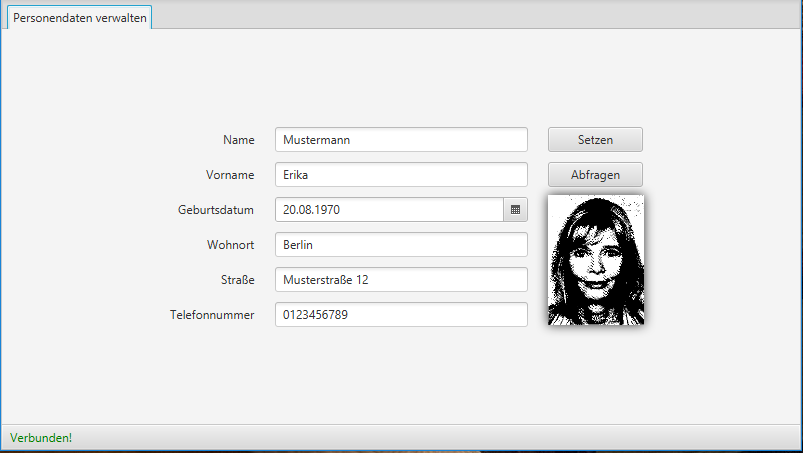
\includegraphics[width=0.9\textwidth]{img/pers}
	\caption{Administration der Personendaten}
	\label{pers}
\end{figure}

Nach dem Betätigen des Sende-Buttons werden alle Felder, sowie das Bild einzeln zur Karte gesendet. Gleiches gilt für die Abfrage der Daten.	
	

\section{Zusammenfassung \& Fazit}

\end{document}
